\documentclass[12pt,a4paper]{article}

\usepackage[a4paper,text={16.5cm,25.2cm},centering]{geometry}
\usepackage{lmodern}
\usepackage{amssymb,amsmath}
\usepackage{bm}
\usepackage{graphicx}
\setkeys{Gin}{width=\linewidth,keepaspectratio}
\usepackage{microtype}
\usepackage{hyperref}
\setlength{\parindent}{0pt}
\setlength{\parskip}{1.2ex}

\hypersetup
       {   pdfauthor = { Austin Shank },
           pdftitle={ Ritz Method — Gelfand - Fomin Problem 8.4 },
           colorlinks=TRUE,
           linkcolor=black,
           citecolor=blue,
           urlcolor=blue
       }

\title{ Ritz Method — Gelfand - Fomin Problem 8.4 }

\author{ Austin Shank }

\date{ 2026-08-14 }

\usepackage{upquote}
\usepackage{listings}
\usepackage{xcolor}
\lstset{
    basicstyle=\ttfamily\footnotesize,
    upquote=true,
    breaklines=true,
    breakindent=0pt,
    keepspaces=true,
    showspaces=false,
    columns=fullflexible,
    showtabs=false,
    showstringspaces=false,
    escapeinside={(*@}{@*)},
    extendedchars=true,
}
\newcommand{\HLJLt}[1]{#1}
\newcommand{\HLJLw}[1]{#1}
\newcommand{\HLJLe}[1]{#1}
\newcommand{\HLJLeB}[1]{#1}
\newcommand{\HLJLo}[1]{#1}
\newcommand{\HLJLk}[1]{\textcolor[RGB]{148,91,176}{\textbf{#1}}}
\newcommand{\HLJLkc}[1]{\textcolor[RGB]{59,151,46}{\textit{#1}}}
\newcommand{\HLJLkd}[1]{\textcolor[RGB]{214,102,97}{\textit{#1}}}
\newcommand{\HLJLkn}[1]{\textcolor[RGB]{148,91,176}{\textbf{#1}}}
\newcommand{\HLJLkp}[1]{\textcolor[RGB]{148,91,176}{\textbf{#1}}}
\newcommand{\HLJLkr}[1]{\textcolor[RGB]{148,91,176}{\textbf{#1}}}
\newcommand{\HLJLkt}[1]{\textcolor[RGB]{148,91,176}{\textbf{#1}}}
\newcommand{\HLJLn}[1]{#1}
\newcommand{\HLJLna}[1]{#1}
\newcommand{\HLJLnb}[1]{#1}
\newcommand{\HLJLnbp}[1]{#1}
\newcommand{\HLJLnc}[1]{#1}
\newcommand{\HLJLncB}[1]{#1}
\newcommand{\HLJLnd}[1]{\textcolor[RGB]{214,102,97}{#1}}
\newcommand{\HLJLne}[1]{#1}
\newcommand{\HLJLneB}[1]{#1}
\newcommand{\HLJLnf}[1]{\textcolor[RGB]{66,102,213}{#1}}
\newcommand{\HLJLnfm}[1]{\textcolor[RGB]{66,102,213}{#1}}
\newcommand{\HLJLnp}[1]{#1}
\newcommand{\HLJLnl}[1]{#1}
\newcommand{\HLJLnn}[1]{#1}
\newcommand{\HLJLno}[1]{#1}
\newcommand{\HLJLnt}[1]{#1}
\newcommand{\HLJLnv}[1]{#1}
\newcommand{\HLJLnvc}[1]{#1}
\newcommand{\HLJLnvg}[1]{#1}
\newcommand{\HLJLnvi}[1]{#1}
\newcommand{\HLJLnvm}[1]{#1}
\newcommand{\HLJLl}[1]{#1}
\newcommand{\HLJLld}[1]{\textcolor[RGB]{148,91,176}{\textit{#1}}}
\newcommand{\HLJLs}[1]{\textcolor[RGB]{201,61,57}{#1}}
\newcommand{\HLJLsa}[1]{\textcolor[RGB]{201,61,57}{#1}}
\newcommand{\HLJLsb}[1]{\textcolor[RGB]{201,61,57}{#1}}
\newcommand{\HLJLsc}[1]{\textcolor[RGB]{201,61,57}{#1}}
\newcommand{\HLJLsd}[1]{\textcolor[RGB]{201,61,57}{#1}}
\newcommand{\HLJLsdB}[1]{\textcolor[RGB]{201,61,57}{#1}}
\newcommand{\HLJLsdC}[1]{\textcolor[RGB]{201,61,57}{#1}}
\newcommand{\HLJLse}[1]{\textcolor[RGB]{59,151,46}{#1}}
\newcommand{\HLJLsh}[1]{\textcolor[RGB]{201,61,57}{#1}}
\newcommand{\HLJLsi}[1]{#1}
\newcommand{\HLJLso}[1]{\textcolor[RGB]{201,61,57}{#1}}
\newcommand{\HLJLsr}[1]{\textcolor[RGB]{201,61,57}{#1}}
\newcommand{\HLJLss}[1]{\textcolor[RGB]{201,61,57}{#1}}
\newcommand{\HLJLssB}[1]{\textcolor[RGB]{201,61,57}{#1}}
\newcommand{\HLJLnB}[1]{\textcolor[RGB]{59,151,46}{#1}}
\newcommand{\HLJLnbB}[1]{\textcolor[RGB]{59,151,46}{#1}}
\newcommand{\HLJLnfB}[1]{\textcolor[RGB]{59,151,46}{#1}}
\newcommand{\HLJLnh}[1]{\textcolor[RGB]{59,151,46}{#1}}
\newcommand{\HLJLni}[1]{\textcolor[RGB]{59,151,46}{#1}}
\newcommand{\HLJLnil}[1]{\textcolor[RGB]{59,151,46}{#1}}
\newcommand{\HLJLnoB}[1]{\textcolor[RGB]{59,151,46}{#1}}
\newcommand{\HLJLoB}[1]{\textcolor[RGB]{102,102,102}{\textbf{#1}}}
\newcommand{\HLJLow}[1]{\textcolor[RGB]{102,102,102}{\textbf{#1}}}
\newcommand{\HLJLp}[1]{#1}
\newcommand{\HLJLc}[1]{\textcolor[RGB]{153,153,119}{\textit{#1}}}
\newcommand{\HLJLch}[1]{\textcolor[RGB]{153,153,119}{\textit{#1}}}
\newcommand{\HLJLcm}[1]{\textcolor[RGB]{153,153,119}{\textit{#1}}}
\newcommand{\HLJLcp}[1]{\textcolor[RGB]{153,153,119}{\textit{#1}}}
\newcommand{\HLJLcpB}[1]{\textcolor[RGB]{153,153,119}{\textit{#1}}}
\newcommand{\HLJLcs}[1]{\textcolor[RGB]{153,153,119}{\textit{#1}}}
\newcommand{\HLJLcsB}[1]{\textcolor[RGB]{153,153,119}{\textit{#1}}}
\newcommand{\HLJLg}[1]{#1}
\newcommand{\HLJLgd}[1]{#1}
\newcommand{\HLJLge}[1]{#1}
\newcommand{\HLJLgeB}[1]{#1}
\newcommand{\HLJLgh}[1]{#1}
\newcommand{\HLJLgi}[1]{#1}
\newcommand{\HLJLgo}[1]{#1}
\newcommand{\HLJLgp}[1]{#1}
\newcommand{\HLJLgs}[1]{#1}
\newcommand{\HLJLgsB}[1]{#1}
\newcommand{\HLJLgt}[1]{#1}


\begin{document}

\maketitle

\section{Problem Statement}
\begin{figure}
\centering
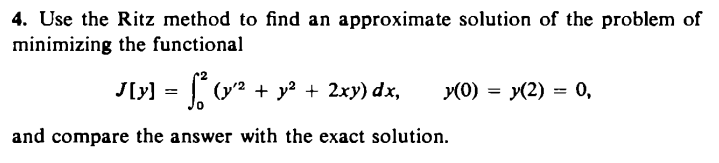
\includegraphics{../imgs/gelfand-fomin_8_4.png}
\caption{Problem 8.4}
\end{figure}


\section{Solution}
\subsection{Exact Solution}
\begin{figure}
\centering
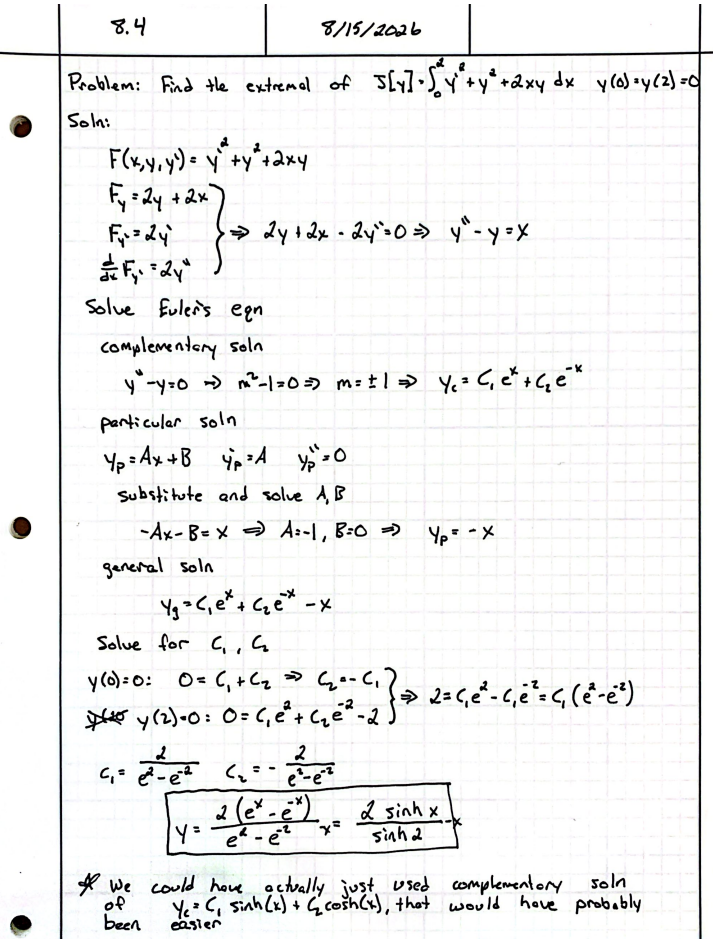
\includegraphics{../imgs/exact_soln_8_4.png}
\caption{Problem 8.2}
\end{figure}
 We will define the julia function of this for comparison against the approximations


\begin{lstlisting}
(*@\HLJLnf{y{\_}exact}@*)(*@\HLJLp{(}@*)(*@\HLJLn{x}@*)(*@\HLJLp{)}@*) (*@\HLJLoB{=}@*) (*@\HLJLni{2}@*) (*@\HLJLoB{*}@*) (*@\HLJLnf{sinh}@*)(*@\HLJLp{(}@*)(*@\HLJLn{x}@*)(*@\HLJLp{)}@*) (*@\HLJLoB{/}@*) (*@\HLJLnf{sinh}@*)(*@\HLJLp{(}@*)(*@\HLJLni{2}@*)(*@\HLJLp{)}@*) (*@\HLJLoB{-}@*) (*@\HLJLn{x}@*)
(*@\HLJLn{have{\_}exact}@*) (*@\HLJLoB{=}@*) (*@\HLJLoB{!}@*)(*@\HLJLnf{isnothing}@*)(*@\HLJLp{(}@*)(*@\HLJLn{y{\_}exact}@*)(*@\HLJLp{)}@*)
\end{lstlisting}


\subsection{Ritz Approximations}
We will use the \texttt{RitzMethod} package


\begin{lstlisting}
(*@\HLJLk{using}@*) (*@\HLJLn{RitzMethod}@*)
(*@\HLJLk{import}@*) (*@\HLJLn{Optim}@*)
(*@\HLJLk{import}@*) (*@\HLJLn{Plots}@*)

(*@\HLJLcs{{\#}}@*) (*@\HLJLcs{Define}@*) (*@\HLJLcs{problem}@*) (*@\HLJLcs{and}@*) (*@\HLJLcs{basis}@*)
(*@\HLJLnf{integrand}@*)(*@\HLJLp{(}@*)(*@\HLJLn{x}@*)(*@\HLJLp{,}@*) (*@\HLJLn{y}@*)(*@\HLJLp{,}@*) (*@\HLJLn{y{\_}prime}@*)(*@\HLJLp{)}@*) (*@\HLJLoB{=}@*) (*@\HLJLn{y{\_}prime}@*)(*@\HLJLoB{{\textasciicircum}}@*)(*@\HLJLni{2}@*) (*@\HLJLoB{+}@*) (*@\HLJLn{y}@*)(*@\HLJLoB{{\textasciicircum}}@*)(*@\HLJLni{2}@*) (*@\HLJLoB{+}@*) (*@\HLJLni{2}@*) (*@\HLJLoB{*}@*) (*@\HLJLn{x}@*) (*@\HLJLoB{*}@*) (*@\HLJLn{y}@*)
(*@\HLJLn{domain}@*) (*@\HLJLoB{=}@*) (*@\HLJLnf{Interval}@*)(*@\HLJLp{(}@*)(*@\HLJLnfB{0.0}@*)(*@\HLJLp{,}@*) (*@\HLJLnfB{2.0}@*)(*@\HLJLp{)}@*)
(*@\HLJLn{full{\_}basis}@*) (*@\HLJLoB{=}@*) (*@\HLJLp{[}@*)(*@\HLJLn{x}@*) (*@\HLJLoB{->}@*) (*@\HLJLn{x}@*)(*@\HLJLoB{{\textasciicircum}}@*)(*@\HLJLn{k}@*) (*@\HLJLoB{*}@*) (*@\HLJLp{(}@*)(*@\HLJLni{2}@*) (*@\HLJLoB{-}@*) (*@\HLJLn{x}@*)(*@\HLJLp{)}@*) (*@\HLJLk{for}@*) (*@\HLJLn{k}@*) (*@\HLJLkp{in}@*) (*@\HLJLni{1}@*)(*@\HLJLoB{:}@*)(*@\HLJLni{3}@*)(*@\HLJLp{]}@*)

(*@\HLJLk{function}@*) (*@\HLJLnf{solve{\_}ritz}@*)(*@\HLJLp{(}@*)(*@\HLJLn{n{\_}terms}@*)(*@\HLJLp{)}@*)
    (*@\HLJLnf{minimizefunctional}@*)(*@\HLJLp{(}@*)
        (*@\HLJLn{integrand}@*)(*@\HLJLp{,}@*) (*@\HLJLn{domain}@*)(*@\HLJLp{,}@*) (*@\HLJLn{full{\_}basis}@*)(*@\HLJLp{[}@*)(*@\HLJLni{1}@*)(*@\HLJLoB{:}@*)(*@\HLJLn{n{\_}terms}@*)(*@\HLJLp{];}@*)
        (*@\HLJLn{num{\_}quad{\_}nodes}@*)(*@\HLJLoB{=}@*)(*@\HLJLni{5}@*)(*@\HLJLp{,}@*)
        (*@\HLJLn{method}@*)(*@\HLJLoB{=}@*)(*@\HLJLn{Optim}@*)(*@\HLJLoB{.}@*)(*@\HLJLnf{BFGS}@*)(*@\HLJLp{(),}@*)
        (*@\HLJLn{options}@*)(*@\HLJLoB{=}@*)(*@\HLJLn{Optim}@*)(*@\HLJLoB{.}@*)(*@\HLJLnf{Options}@*)(*@\HLJLp{(}@*)(*@\HLJLn{iterations}@*)(*@\HLJLoB{=}@*)(*@\HLJLni{50}@*)(*@\HLJLp{,}@*) (*@\HLJLn{g{\_}abstol}@*)(*@\HLJLoB{=}@*)(*@\HLJLnfB{1e-20}@*)(*@\HLJLp{,}@*) (*@\HLJLn{x{\_}reltol}@*)(*@\HLJLoB{=}@*)(*@\HLJLnfB{1e-8}@*)(*@\HLJLp{),}@*)
    (*@\HLJLp{)}@*)
(*@\HLJLk{end}@*)

(*@\HLJLn{results}@*) (*@\HLJLoB{=}@*) (*@\HLJLp{[}@*)(*@\HLJLnf{solve{\_}ritz}@*)(*@\HLJLp{(}@*)(*@\HLJLn{n}@*)(*@\HLJLp{)}@*) (*@\HLJLk{for}@*) (*@\HLJLn{n}@*) (*@\HLJLkp{in}@*) (*@\HLJLni{1}@*)(*@\HLJLoB{:}@*)(*@\HLJLni{3}@*)(*@\HLJLp{]}@*)
\end{lstlisting}


\subsubsection{One-Term Approximation}

\begin{lstlisting}
(*@\HLJLnf{println}@*)(*@\HLJLp{(}@*)(*@\HLJLnf{summarize}@*)(*@\HLJLp{(}@*)(*@\HLJLn{results}@*)(*@\HLJLp{[}@*)(*@\HLJLni{1}@*)(*@\HLJLp{]))}@*)
\end{lstlisting}

\begin{lstlisting}
RitzResult:
  Domain:          [0.0, 2.0]
  Coefficients:    [-0.35714285714285726]
  Minimized value: -0.47619047619047633
  Converged:       true
\end{lstlisting}


\subsubsection{Two-Term Approximation}

\begin{lstlisting}
(*@\HLJLnf{println}@*)(*@\HLJLp{(}@*)(*@\HLJLnf{summarize}@*)(*@\HLJLp{(}@*)(*@\HLJLn{results}@*)(*@\HLJLp{[}@*)(*@\HLJLni{2}@*)(*@\HLJLp{]))}@*)
\end{lstlisting}

\begin{lstlisting}
RitzResult:
  Domain:          [0.0, 2.0]
  Coefficients:    [-0.20496894409937896, -0.15217391304347833]
  Minimized value: -0.5167701863354041
  Converged:       true
\end{lstlisting}


\subsubsection{Three-Term Approximation}

\begin{lstlisting}
(*@\HLJLnf{println}@*)(*@\HLJLp{(}@*)(*@\HLJLnf{summarize}@*)(*@\HLJLp{(}@*)(*@\HLJLn{results}@*)(*@\HLJLp{[}@*)(*@\HLJLni{3}@*)(*@\HLJLp{]))}@*)
\end{lstlisting}

\begin{lstlisting}
RitzResult:
  Domain:          [0.0, 2.0]
  Coefficients:    [-0.22826086956521813, -0.09510869565217232, -0.02853260
869565301]
  Minimized value: -0.5173913043478264
  Converged:       true
\end{lstlisting}


\section{Comparison}

\begin{lstlisting}
Term count | Minimized J[y] | Coefficients
1          | -0.47619048    | [-0.35714285714285726]
2          | -0.51677019    | [-0.20496894409937896, -0.15217391304347833]
3          | -0.51739130    | [-0.22826086956521813, -0.09510869565217232, 
-0.02853260869565301]
\end{lstlisting}


\begin{figure}[!h]
\center
\includegraphics[width=\linewidth]{jl_Z1VA2e/report_7_1.pdf}
\caption{Ritz Approximations}
\end{figure}

\section{Approximation Error}

\begin{figure}[!h]
\center
\includegraphics[width=\linewidth]{jl_Z1VA2e/report_8_1.pdf}
\caption{Pointwise error between Ritz approximations and the exact solution.}
\end{figure}


\end{document}
